% Options for packages loaded elsewhere
\PassOptionsToPackage{unicode}{hyperref}
\PassOptionsToPackage{hyphens}{url}
%
\documentclass[
]{article}
\usepackage{lmodern}
\usepackage{amssymb,amsmath}
\usepackage{ifxetex,ifluatex}
\ifnum 0\ifxetex 1\fi\ifluatex 1\fi=0 % if pdftex
  \usepackage[T1]{fontenc}
  \usepackage[utf8]{inputenc}
  \usepackage{textcomp} % provide euro and other symbols
\else % if luatex or xetex
  \usepackage{unicode-math}
  \defaultfontfeatures{Scale=MatchLowercase}
  \defaultfontfeatures[\rmfamily]{Ligatures=TeX,Scale=1}
\fi
% Use upquote if available, for straight quotes in verbatim environments
\IfFileExists{upquote.sty}{\usepackage{upquote}}{}
\IfFileExists{microtype.sty}{% use microtype if available
  \usepackage[]{microtype}
  \UseMicrotypeSet[protrusion]{basicmath} % disable protrusion for tt fonts
}{}
\makeatletter
\@ifundefined{KOMAClassName}{% if non-KOMA class
  \IfFileExists{parskip.sty}{%
    \usepackage{parskip}
  }{% else
    \setlength{\parindent}{0pt}
    \setlength{\parskip}{6pt plus 2pt minus 1pt}}
}{% if KOMA class
  \KOMAoptions{parskip=half}}
\makeatother
\usepackage{xcolor}
\IfFileExists{xurl.sty}{\usepackage{xurl}}{} % add URL line breaks if available
\IfFileExists{bookmark.sty}{\usepackage{bookmark}}{\usepackage{hyperref}}
\hypersetup{
  pdftitle={Ejercicio 2},
  hidelinks,
  pdfcreator={LaTeX via pandoc}}
\urlstyle{same} % disable monospaced font for URLs
\usepackage[margin=1in]{geometry}
\usepackage{graphicx,grffile}
\makeatletter
\def\maxwidth{\ifdim\Gin@nat@width>\linewidth\linewidth\else\Gin@nat@width\fi}
\def\maxheight{\ifdim\Gin@nat@height>\textheight\textheight\else\Gin@nat@height\fi}
\makeatother
% Scale images if necessary, so that they will not overflow the page
% margins by default, and it is still possible to overwrite the defaults
% using explicit options in \includegraphics[width, height, ...]{}
\setkeys{Gin}{width=\maxwidth,height=\maxheight,keepaspectratio}
% Set default figure placement to htbp
\makeatletter
\def\fps@figure{htbp}
\makeatother
\setlength{\emergencystretch}{3em} % prevent overfull lines
\providecommand{\tightlist}{%
  \setlength{\itemsep}{0pt}\setlength{\parskip}{0pt}}
\setcounter{secnumdepth}{-\maxdimen} % remove section numbering
\usepackage{float}
\usepackage{booktabs}
\usepackage{longtable}
\usepackage{array}
\usepackage{multirow}
\usepackage{wrapfig}
\usepackage{colortbl}
\usepackage{pdflscape}
\usepackage{tabu}
\usepackage{threeparttable}
\usepackage{threeparttablex}
\usepackage[normalem]{ulem}
\usepackage{makecell}
\usepackage{xcolor}

\title{Ejercicio 2}
\author{}
\date{\vspace{-2.5em}}

\begin{document}
\maketitle

Los datos del archivo QUINOA corresponden a 24 accesiones de quinoa
nativa del Noroeste Argentino conservadas en el Banco de Germoplasma,
caracterizadas a través de 10 variables cuantitativas y 8 variables
cualitativas. En el identificador de cada accesión se encuentra la
indicación de la procedencia del mismo: AL (altiplano), VA (Valles de
altura), VS (Valles secos), VH (Valles húmedos orientales).

\hypertarget{variables-cuantitativas}{%
\section{Variables cuantitativas:}\label{variables-cuantitativas}}

\begin{itemize}
\tightlist
\item
  DIAMTAL Diámetro del tallo (mm)
\item
  ALTPL Altura de planta (cm)
\item
  LONGHO Longitud de la hoja (mm)
\item
  ANCHOHO Ancho de la hoja (mm)
\item
  LONGPEC Longitud del peciolo (mm)
\item
  LONGPAN Longitud de la panoja (cm)
\item
  LONGGLO Longitud del glomérulo (mm)
\item
  DSBF Días desde siembra a botón floral (días)
\item
  DSFL Días desde siembra a floración (días)
\item
  DSMF Días desde siembra a madurez fisiológica (días)
\end{itemize}

\hypertarget{variables-cualitativas}{%
\section{Variables cualitativas:}\label{variables-cualitativas}}

\begin{itemize}
\tightlist
\item
  AX Presencia de axilas: Si -- No
\item
  CEstrias Color de las estrías: amarilla, rojas, purpuras, no (no tiene
  estrías)
\item
  CTallo Color del tallo: rojo, púrpura, verde
\item
  PoRAMA Presencia de ramas Si -- No
\item
  CFA Color de panoja a fin de antesis: Blanca -- Púrpura -- Gris
\item
  Cco Color de la panoja a la cosecha: amarilla, blanca, púrpura, marrón
\item
  TP Tipo de panoja: Diferenciada y terminal -- No diferenciada
\item
  FP Forma de panoja: Glomerulada -- Amarantiforme
\end{itemize}

\hypertarget{origen-de-los-individuos}{%
\section{Origen de los individuos}\label{origen-de-los-individuos}}

\begin{itemize}
\tightlist
\item
  AL Altiplano
\item
  VA Valles de altura
\item
  VH Valles húmedos
\item
  VS Valles secos
\end{itemize}

\begin{enumerate}
\def\labelenumi{\Alph{enumi})}
\item
\begin{verbatim}
 Realice un ACP con las variables cuantitativas.
\end{verbatim}
\end{enumerate}

\begin{verbatim}
##       DIAMTAL ALTPL   LONGHO  ANCHOHO  LONGPEC LONGPAN LONGGLO DSBF DSFL DSMF
## AL420   4.161 34.36 37.99333 33.57333 16.44667 148.500   7.468   18   39  115
## AL426   3.359 29.20 36.68333 32.75333 16.87667 120.600   5.121   21   36   88
## AL427   2.926 23.20 65.53333 46.20667 36.09667  50.740   6.912   18   33  123
## AL431   3.369 33.02 48.31667 37.99333 31.37000 144.000   6.505   21   42  124
## AL432   3.877 41.42 55.31333 36.77000 21.23667 116.212   5.705   23   41  120
## AL438   2.803 28.18 66.64333 45.54000 34.02833 114.000  11.148   18   36   93
##         AX CEstrias CTallo PoRAMA   CFA   Cco      TP     FP
## AL420 AxNo   CEstAm  CTaVe PoRaNo CFAbl CcoAm   TPDif  FPAma
## AL426 AxNo   CEstRo  CTaVe PoRaNo CFAbl CcoAm   TPDif FPGlom
## AL427 AxSi   CEstRo  CTaVe PoRaBa CFAbl CcoGr TPNoDif FPGlom
## AL431 AxNo   CEstRo  CTaVe PoRaNo CFAbl CcoAm   TPDif FPGlom
## AL432 AxSi   CEstRo  CTaVe PoRaOb CFAbl CcoAm TPNoDif FPGlom
## AL438 AxSi   CEstRo  CTaVe PoRaNo CFAbl CcoAm   TPDif FPGlom
\end{verbatim}

\begin{center}\includegraphics{parte_2_files/figure-latex/unnamed-chunk-3-1} \end{center}

\begin{verbatim}
Luego de realizar el analisis de componentes principales, podemos observar que el porcentaje de           variabilidad total explicada por las dos primeras componentes es de 81.31%; el      68.09% corresponde a la primera componente, mientras que el 
13.22% restante corresponde a la segunda componente.
\end{verbatim}

\begin{center}\includegraphics{parte_2_files/figure-latex/unnamed-chunk-4-1} \end{center}

\begin{verbatim}
En relacion a las variables que mas aportan a la formacion de las componentes, podemos decir que todas las variables contribuyen de forma positiva a la primer componente, pero Longitud del glomérulo lo hace en menor medida.
Con respecto a la Segunda Componente, podemos decir que las variables que mas aportan son Longitud y 
Ancho de la hoja (de forma positiva) y días desde siembra a botón floral y a floración (de forma          negativa)
\end{verbatim}

\begin{center}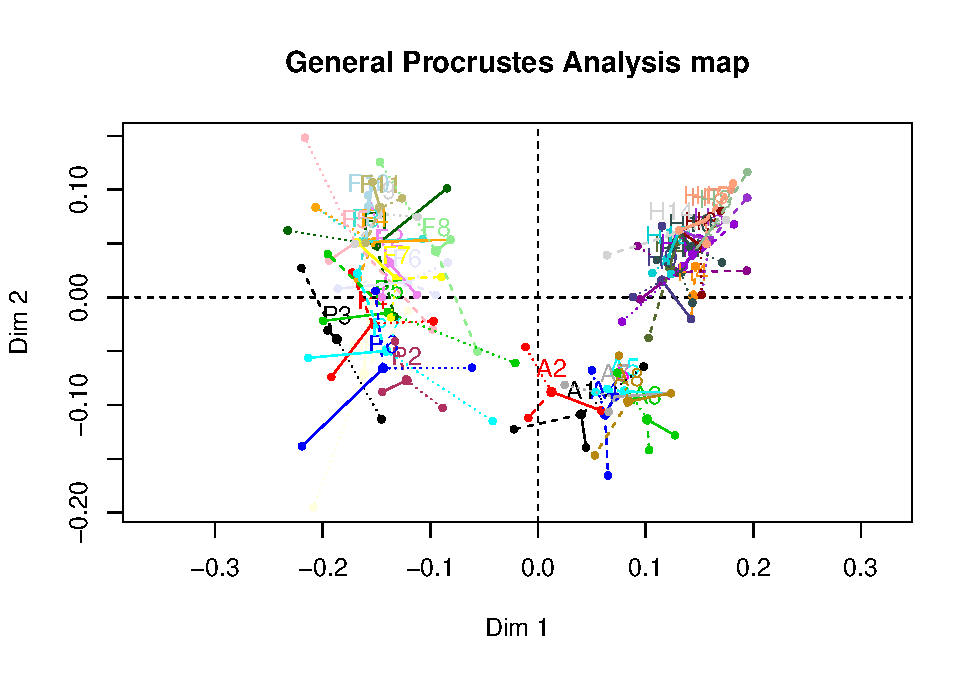
\includegraphics{parte_2_files/figure-latex/unnamed-chunk-5-1} \end{center}

\begin{verbatim}
    La figura anterior permite caracterizar a las distintas accesiones de Quinoa sobre el plano principal de las dos primeras componentes. En la misma, podemos observar que las de Altiplano poseen valores bajos de la Primer Componente, distinguiendose de los Valles. 
    Las correspondientes a Valles Seco y Humedo forman un solo grupo y no se logra diferenciar entre ellos. Estas accesiones poseen valores altos de la Primer Componente.
    Con respecto a Valles de Altura, podemos decir que poseen mucha variabilidad sobre la Segunda             Componente
\end{verbatim}

\begin{enumerate}
\def\labelenumi{\Alph{enumi})}
\item
\begin{verbatim}
 Realice un ACM con las variables cualitativas y compare las configuraciones de individuos provistas por ambas técnicas en el plano principal.
\end{verbatim}
\end{enumerate}

\begin{center}\includegraphics{parte_2_files/figure-latex/unnamed-chunk-6-1} \end{center}

\begin{verbatim}
El porcentaje de incercia explicado es de 42.39%, siendo bastante menor que lo        obtenido con ACP. Este resultado es alentador, ya que nos indica que al incorporar nueva informacion      acerca de caracteristicas Cualitativas de la Quinoa el analisis puede ser enriquecido.
\end{verbatim}

\begin{center}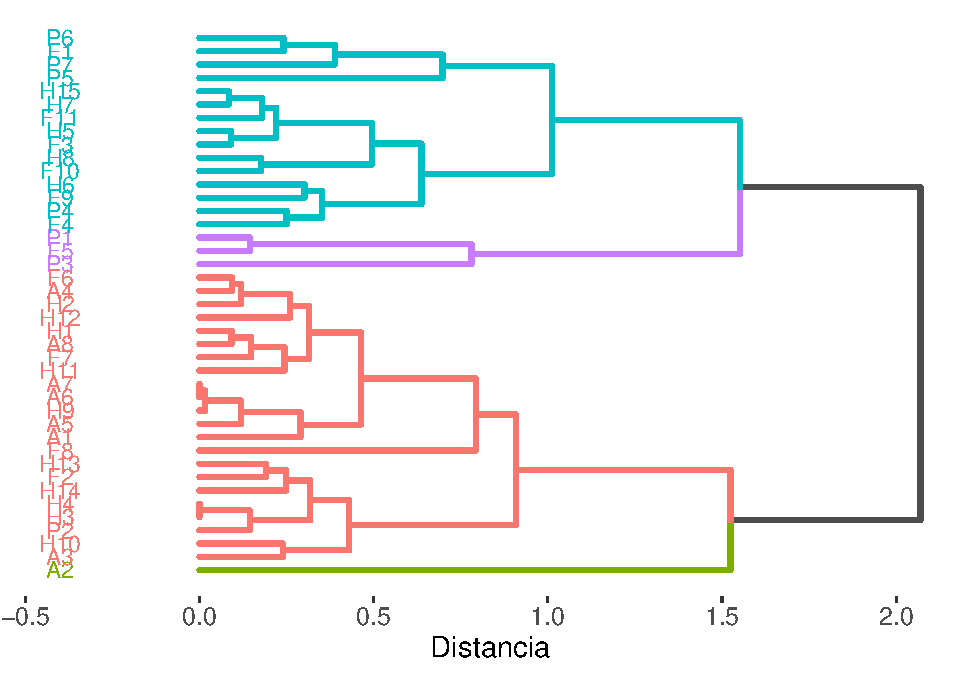
\includegraphics{parte_2_files/figure-latex/unnamed-chunk-7-1} \end{center}

\begin{verbatim}
Las variables que mas aportan a la formacion del Eje 1 son Color de las estrias, Color de 
panoja a fin de antesis y Color de tallo; mientras que Color de la panoja a la cosecha y Tipo 
de panoja son las que mas contribuyen al Eje 2.
\end{verbatim}

\begin{center}\includegraphics{parte_2_files/figure-latex/unnamed-chunk-8-1} \end{center}

\begin{verbatim}
Al observar el grafico anterior, donde se representan los "individuos" sobre los dos primeros ejes 
principales, no se logra distinguir a los ambientes; es decir las variables cualitativas, a diferencia
de las cuantitativas, no logran diferenciarlos.

Luego, si comparamos las configuraciones de individuos provistas por las dos tecnicas realizadas,         podemos concluir que las mismas parecen no ser homogeneas, ya que, como se pudo observar, una tecnica     logra una diferenciacion por ambientes mientras que la otra no.
\end{verbatim}

\#Con alguna tecnica numerica podriamos realizar esa comparacion: \#Para
poder comparar, siempre en el plano principal, en acp, se podría buscar
una matriz de distancias euclideas entre individuos, lo mismo puedo tmb
hacer para acm. Luego, puedo comparar esas matrices de distancia, medir
el ``acuerdo'', a traves de una corr de matrices de distancias(tiene que
dar un valor bajo)

\hypertarget{realice-un-afm-considerando-como-grupos-a-ambos-tipos-de-variables}{%
\subsection{Realice un AFM considerando como grupos a ambos tipos de
variables:}\label{realice-un-afm-considerando-como-grupos-a-ambos-tipos-de-variables}}

\begin{enumerate}
\def\labelenumi{\alph{enumi})}
\setcounter{enumi}{2}
\tightlist
\item
  Realice el análisis de la interestructura. ¿Qué puede decir de la
  relación existe entre los grupos?
\end{enumerate}

\begin{table}[H]

\caption{\label{tab:unnamed-chunk-10}Coeficiente Lg}
\centering
\fontsize{10}{12}\selectfont
\begin{tabular}[t]{l|c|c|c}
\hline
  & Cuantitativas & Cualitativas & MFA\\
\hline
Cuantitativas & 1.06 & 0.23 & 1.11\\
\hline
Cualitativas & 0.23 & 1.92 & 1.85\\
\hline
MFA & 1.11 & 1.85 & 2.55\\
\hline
\end{tabular}
\end{table}

\begin{verbatim}
Al obtener el Coeficiente Lg, el cual nos brinda una medida de estructura comun entre las variables       Caulitativas y Cuantitativas, observamos que el mismo es de 0.23. Dado que      se obtuvo un valor bajo, podemos decir que las variables del grupo "Cuantitativas" no estan               correlacionadas con las del grupo "Cualitativas". Es decir, las configuraciones no tienen estructura      en comun.
\end{verbatim}

\begin{table}[H]

\caption{\label{tab:unnamed-chunk-11}Coeficiente Ng}
\centering
\fontsize{10}{12}\selectfont
\begin{tabular}[t]{l|c|c|c}
\hline
  & Cuantitativas & Cualitativas & MFA\\
\hline
Cuantitativas & 1.03 & 0.48 & 1.05\\
\hline
Cualitativas & 0.48 & 1.39 & 1.36\\
\hline
MFA & 1.05 & 1.36 & 1.60\\
\hline
\end{tabular}
\end{table}

\begin{verbatim}
Al obtener una medida de dimensionalidad de cada grupo (coeficiente Ng), observamos que el grupo         "Cualitativas" tiene una dimensionalidad mayor que "Cuantitativas"
\end{verbatim}

\begin{table}[H]

\caption{\label{tab:unnamed-chunk-12}Coeficiente RV}
\centering
\fontsize{10}{12}\selectfont
\begin{tabular}[t]{l|c|c|c}
\hline
  & Cuantitativas & Cualitativas & MFA\\
\hline
Cuantitativas & 1.00 & 0.16 & 0.68\\
\hline
Cualitativas & 0.16 & 1.00 & 0.84\\
\hline
MFA & 0.68 & 0.84 & 1.00\\
\hline
\end{tabular}
\end{table}

\begin{verbatim}
Tal como se intuyo al realizar el analisis por separado, las configuraciones cualitativas y               cuantitativas de las quinoas no son "homoteticas" entre si. Luego, al ser un valor bajo indica que los     grupos de variables brindan informacion complementarria.
\end{verbatim}

\begin{figure}[H]

{\centering \includegraphics{parte_2_files/figure-latex/unnamed-chunk-13-1} 

}

\caption{Caracterizacion de los grupos de variables en el plano principal AFM.}\label{fig:unnamed-chunk-13}
\end{figure}

\begin{verbatim}
Si observamos el grafico anterior, podemos ver que las variables Cuantitativas son las que contribuyen     a la formacion de la Coordenada 1, mientras que las Cualitativas son las que contribuyen a la             formacion de la Coordenada 2 del Analisis Factorial Multiple.
\end{verbatim}

\begin{table}[H]

\caption{\label{tab:unnamed-chunk-14}Contribuciones a los Ejes - Cualitativas}
\centering
\fontsize{10}{12}\selectfont
\begin{tabular}[t]{l|c|c}
\hline
  & Dim.1 & Dim.2\\
\hline
AxNo & 0.07 & 3.73\\
\hline
AxSi & 0.12 & 6.22\\
\hline
CEstAm & 0.14 & 0.50\\
\hline
CEstNo & 1.26 & 2.64\\
\hline
CEstPu & 0.74 & 16.54\\
\hline
CEstRo & 2.95 & 0.85\\
\hline
CTaPu & 0.38 & 10.47\\
\hline
CTaRo & 1.44 & 6.63\\
\hline
CTaVe & 0.01 & 2.43\\
\hline
PoRaBa & 0.65 & 0.64\\
\hline
PoRaNo & 0.39 & 1.56\\
\hline
PoRaOb & 0.00 & 3.61\\
\hline
CFAbl & 0.15 & 3.31\\
\hline
CFApu & 0.74 & 16.54\\
\hline
CcoAm & 0.00 & 0.28\\
\hline
CcoBl & 0.26 & 0.54\\
\hline
CcoGr & 2.73 & 0.05\\
\hline
CcoMar & 1.44 & 6.63\\
\hline
CcoPu & 1.95 & 0.97\\
\hline
TPDif & 0.86 & 0.14\\
\hline
TPNoDif & 3.27 & 0.52\\
\hline
FPAma & 0.42 & 4.51\\
\hline
FPGlom & 0.21 & 2.26\\
\hline
\end{tabular}
\end{table}

\begin{table}[H]

\caption{\label{tab:unnamed-chunk-15}Contribuciones a los Ejes - Cuantitativas}
\centering
\fontsize{10}{12}\selectfont
\begin{tabular}[t]{l|c|c}
\hline
  & Dim.1 & Dim.2\\
\hline
DIAMTAL & 9.41 & 0.77\\
\hline
ALTPL & 10.98 & 0.59\\
\hline
LONGHO & 5.48 & 1.79\\
\hline
ANCHOHO & 7.47 & 2.85\\
\hline
LONGPEC & 6.04 & 1.61\\
\hline
LONGPAN & 8.59 & 0.32\\
\hline
LONGGLO & 6.09 & 0.02\\
\hline
DSBF & 8.47 & 0.43\\
\hline
DSFL & 9.97 & 0.04\\
\hline
DSMF & 7.31 & 0.04\\
\hline
\end{tabular}
\end{table}

\begin{enumerate}
\def\labelenumi{\alph{enumi})}
\setcounter{enumi}{3}
\tightlist
\item
  ¿Existe un agrupamiento de individuos por zona?
\end{enumerate}

\begin{center}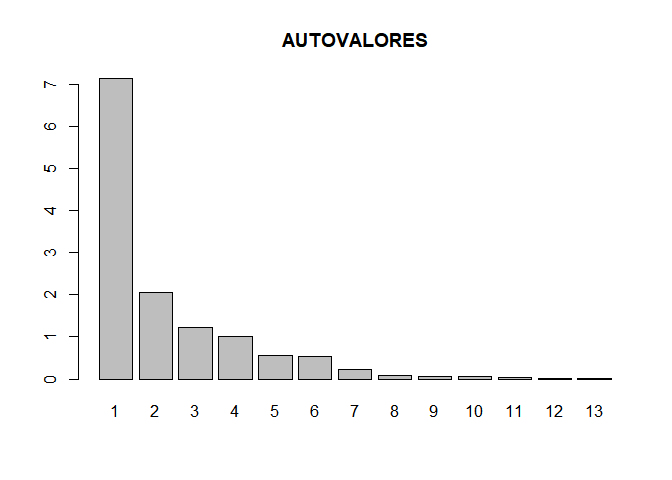
\includegraphics{parte_2_files/figure-latex/unnamed-chunk-16-1} \end{center}

\begin{verbatim}
Vemos que abajo a la izq estan las Altiplano (similar a como habia quedado en las cuali), luego vemos valles humedos y secos juntos. Las de altura estan mas dispersas, y forman dos grupos sobre el eje vertical, lo que estaria indicando que difieren en sus vbles cualitativas, ya q estas vbles son las q contribuyen a la formacion del eje vertical. Podemos ver que hay dos "individuos" (VS414 Y VH458) qson atipicos. Seguramente esto se deba a que tengan valores mas altos de cualitativas, distinto al resto (ya q el eje 2 es cuali) VER!!
\end{verbatim}

\begin{center}\includegraphics{parte_2_files/figure-latex/unnamed-chunk-17-1} \end{center}

\begin{verbatim}
Con este grafico confirmamos lo anterior, VS414 y VH458 poseen valores mas altos de cualitativas q el         resto, es por ello q se apartan del grupo. REDACTAR MEJOR!  
\end{verbatim}

\begin{center}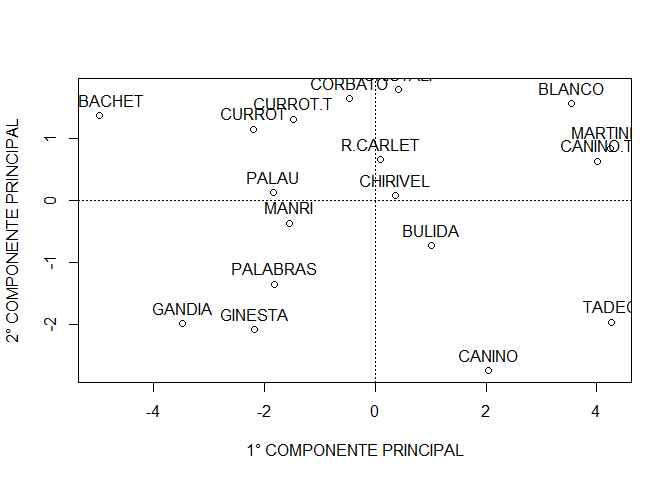
\includegraphics{parte_2_files/figure-latex/unnamed-chunk-18-1} \end{center}

\begin{enumerate}
\def\labelenumi{\alph{enumi})}
\setcounter{enumi}{4}
\item
  Caracterice los grupos de individuos a través de todas las variables.

  con los graficos anteriores caracterizar los grupos y decir cuales
  quinoas tienen hojas mas grandes y bla bla bla
\end{enumerate}

\end{document}
